\documentclass[12pt]{article}    
\usepackage{ucs} 
\usepackage[utf8x]{inputenc}
\usepackage[russian]{babel}  
\usepackage{float}
\title{Псевдоэксперимент №5}
\author{Хафизов Фанис}
\usepackage[pdftex]{graphicx}
\usepackage{multirow}

\begin{document}
	\begin{figure}
		\centering
		
\includegraphics[width=0.3\linewidth]{logo}
	\end{figure}
	\maketitle
	\newpage
	\section{Теоретическая зависимость $\tau(v)$}
	\begin{figure}[H]
		\centering
		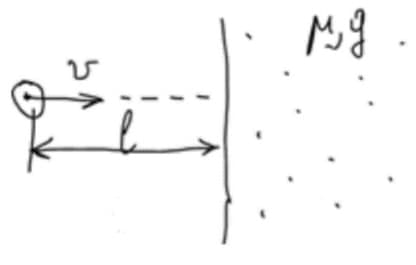
\includegraphics[width=0.5\linewidth]{scheme}
	\end{figure}
	Первую часть пути шайба преодолевает за время $\displaystyle\tau_1=\frac{l}{v}$. Затем она начинает тормозить с ускорением $a = \mu g$. Следовательно, на втором участке шайба остановится через время $\displaystyle\tau_2=\frac{v}{\mu g}$.\\
	Полное время движения $\displaystyle\tau = \tau_1 + \tau_2 = \frac{l}{v} + \frac{v}{\mu g}$.\\
	Заметим, что при $v \gg 1$ $\tau_1\ll 1$ и $\displaystyle\tau \approx \tau_2 = \frac{v}{\mu g}$.\\
	При $v \ll 1$ $\tau_2 \ll 1$ и $\displaystyle\tau \approx \tau_1 = \frac{l}{v}$.
	\section{Нахождение параметров $l$ и $\mu$}
	Разобьем данные на две группы: в первой $v < 1$, во второй -- $v > 1$. Для первой построим график зависимости $\tau(\frac{1}{v})$, для второй -- $\tau(v)$.
	\begin{figure}[H]
		\centering
		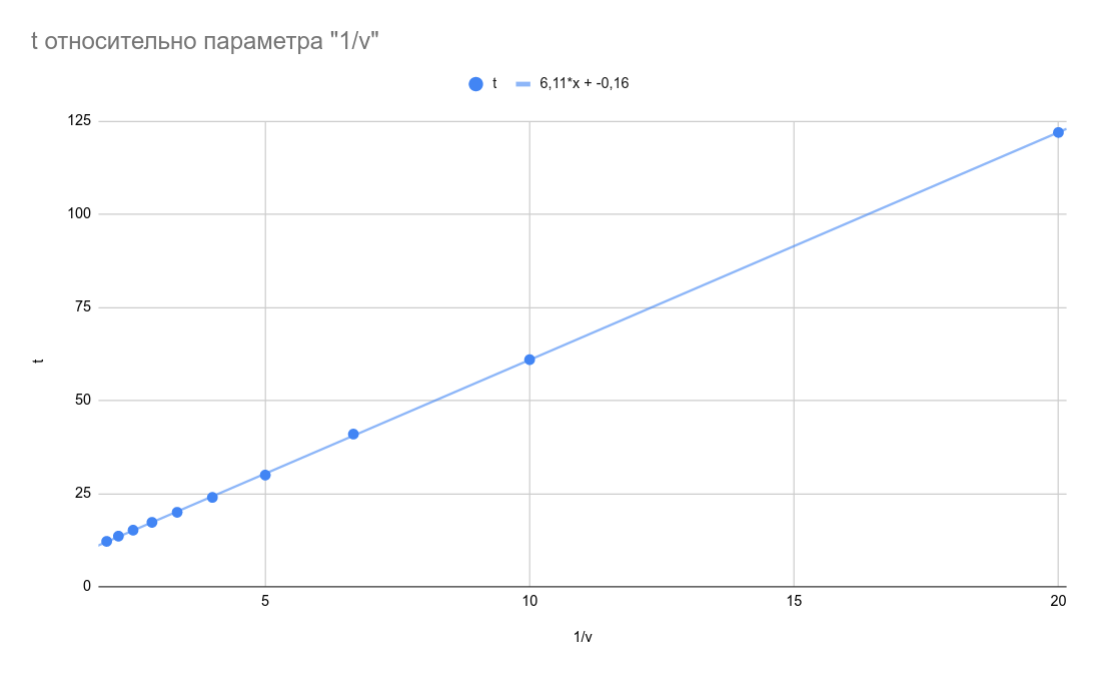
\includegraphics[width=0.9\linewidth]{graph1}
		\caption{График зависимости $\tau(\frac{1}{v})$ при малых $v$}
	\end{figure}
	\begin{figure}[H]
		\centering
		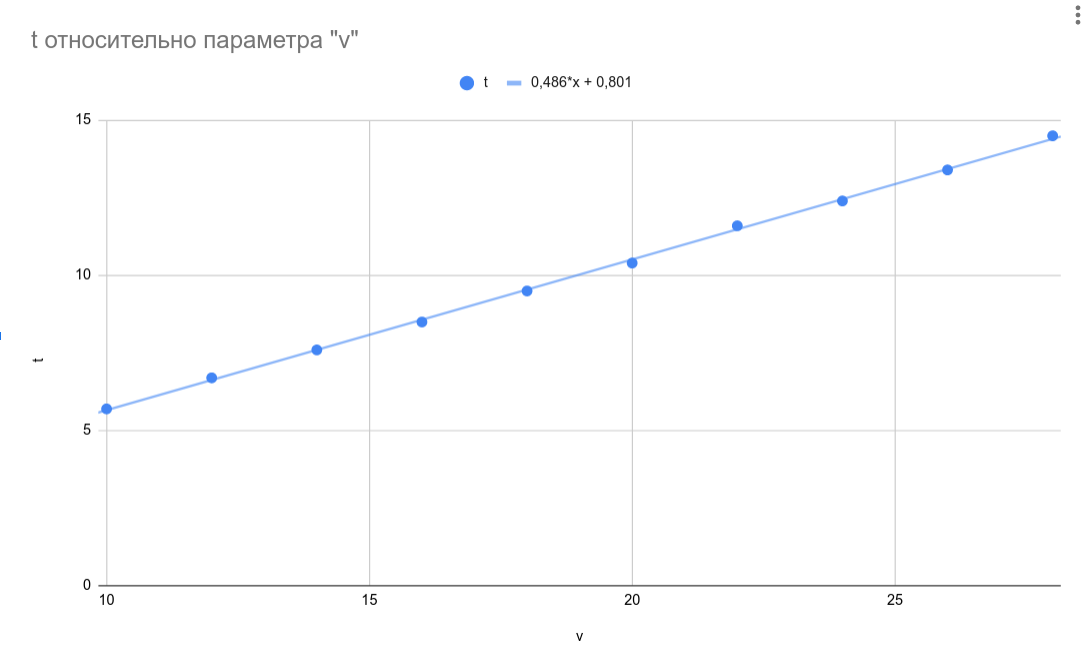
\includegraphics[width=0.9\linewidth]{graph2}
		\caption{График зависимости $\tau(v)$ при больших $v$}
	\end{figure}
	Оба графика получились линейными. Теоретическая зависимость для первого графика $\displaystyle\tau = \frac{l}{v}$. Угловой коэффициент первого графика равен $6{,}11$. $\Rightarrow$ $l = 6{,}11$ м.\\
	Теоретичекская зависимость для второго графика $\displaystyle\tau = \frac{v}{\mu g}$. Угловой коэффициент графика равен $0{,}486$. $\Rightarrow$ $\displaystyle\mu = \frac{1}{0{,}486 g}=\frac{1}{0{,}486\cdot 9{,}8}=0,21$.
	\section{Нахождение $v_{min}$, $\tau_{min}$}
	$$\tau(v) = \frac{l}{v} + \frac{v}{\mu g}$$
	$$\tau'(v) = -\frac{l}{v^2} + \frac{1}{\mu g}$$
	Необходимое условие экстремума -- $\tau'(v) = 0$.
	$$-\frac{l}{v^2} + \frac{1}{\mu g} = 0$$
	$$v = \pm\sqrt{l\mu g}$$
	Так как мы рассматриваем модуль скорости, то берем значение с плюсом.
	$$v_{min} = \sqrt{l\mu g} = \sqrt{\frac{6{,}11}{0{,}486}} = 3{,}55 m/s$$
	$$\tau_{min} = \tau(v_{min}) = \frac{l}{v_{min}} + \frac{v_{min}}{\mu g} = \frac{l}{\sqrt{l\mu g}} + \frac{\sqrt{l\mu g}}{\mu g} = \sqrt{\frac{l}{\mu g}}+\sqrt{\frac{l}{\mu g}} = 2\sqrt{\frac{l}{\mu g}}=2\sqrt{6{,}11\cdot0{,}486} = 3{,}45 s$$
	\section{Результаты}
	$l = 6{,}11$ м\\
	$\mu = 0{,}21$\\
	$v_{min} = 3{,}55$ м/с\\
	$\tau_{min} = 3{,}45$ с
	
\end{document}